\chapter{Image Classification in Practice}
\label{ch:lesson36}

Every classifier so far has been evaluated with a single number: overall accuracy. That number hides a lot. This chapter builds a 4-class classifier on a deliberately imbalanced subset of \textbf{CIFAR-10} (\citelink{krizhevsky2009cifar}{Krizhevsky, 2009}) --- real photographs, not synthetic shapes --- and shows why accuracy alone can be misleading, using the tools that reveal what's actually going wrong: the \textbf{confusion matrix}, and \textbf{per-class precision and recall}.

\section{A 4-class, imbalanced dataset}

Four real photo categories from CIFAR-10: cat, dog, automobile, and truck (Figure~\ref{fig:l36-1}). The test set has an even 150 images per class, but the \emph{training} set is deliberately starved of trucks (90 examples, versus 400 each for the other three) --- a stand-in for the common real-world situation where some classes are just rarer to collect than others. Cat and dog are included deliberately as a visually similar pair, regardless of how much training data either gets.

\begin{figure}[h]
\centering
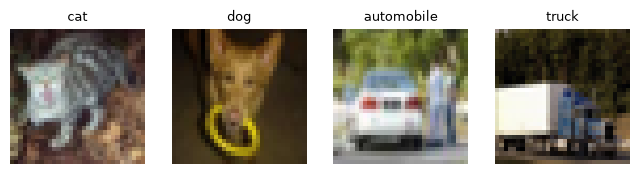
\includegraphics[width=0.7\textwidth]{figures/lesson36_fig01.png}
\caption{One example from each of the four classes.}
\label{fig:l36-1}
\end{figure}

\begin{lstlisting}
class CNN(nn.Module):
    def __init__(self):
        super().__init__()
        self.conv = nn.Sequential(
            nn.Conv2d(3, 16, 5, padding=2), nn.ReLU(), nn.MaxPool2d(2),
            nn.Conv2d(16, 32, 5, padding=2), nn.ReLU(), nn.MaxPool2d(2),
            nn.Conv2d(32, 64, 3, padding=1), nn.ReLU(),
            nn.AdaptiveMaxPool2d(1),
        )
        self.fc = nn.Linear(64, 4)
\end{lstlisting}

Trained for 150 epochs: overall test accuracy is $50.3\%$. Just over 50\% overall accuracy, on a 4-class task where chance is 25\%, sounds like a reasonable result for a small from-scratch CNN on real photos. It hides something important: the model is not equally good at all four classes.

\section{Confusion matrix}

Row $i$, column $j$ counts test examples of true class $i$ predicted as class $j$. A perfect classifier is diagonal; everything off the diagonal is a specific, nameable mistake.

\begin{center}
\renewcommand{\arraystretch}{1.3}
\begin{tabular}{lrrrr}
\hline
\textbf{true \textbackslash\ predicted} & \textbf{cat} & \textbf{dog} & \textbf{automobile} & \textbf{truck} \\
\hline
cat        & 60 & 68 & 20  & 2 \\
dog        & 47 & 95 & 7   & 1 \\
automobile & 9  & 5  & 134 & 2 \\
truck      & 21 & 13 & 103 & 13 \\
\hline
\end{tabular}
\end{center}

\begin{figure}[h]
\centering
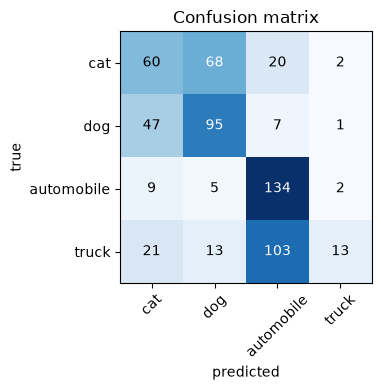
\includegraphics[width=0.45\textwidth]{figures/lesson36_fig02.png}
\caption{The confusion matrix, visualized: rows are true class, columns are predicted class.}
\label{fig:l36-2}
\end{figure}

Figure~\ref{fig:l36-2} makes the pattern jump out immediately: truck's row is scattered everywhere except its own diagonal cell, while automobile's column absorbs a disproportionate share of every other row's mistakes.

\section{True positives, false positives, true negatives, false negatives}

Every cell of the confusion matrix above is a specific kind of correctness or mistake, but the standard vocabulary for talking about them is binary: pick one class and ask only ``is it this, or not?'' Collapsing the 4-class matrix down to ``truck vs.\ everything else'' gives exactly four outcomes:
\begin{itemize}
  \item \textbf{True positive (TP)}: actually a truck, predicted truck. A hit.
  \item \textbf{False negative (FN)}: actually a truck, predicted something else. A miss --- the model let it slip past.
  \item \textbf{False positive (FP)}: actually \emph{not} a truck, predicted truck anyway. A false alarm.
  \item \textbf{True negative (TN)}: actually not a truck, correctly predicted not-truck.
\end{itemize}
This is the same $2\times2$ table underlying every binary classifier's evaluation (a medical test's ``positive/negative'' result, a spam filter's ``spam/not spam'' decision) --- a multi-class confusion matrix is just this table computed once per class, with everything off that class's row/column collapsed into ``not this class.'' For truck: $\text{TP}=13$, $\text{FP}=5$, $\text{FN}=137$, $\text{TN}=445$ (total $600$, matching the test set size).

\section{Precision and recall}

Two numbers per class, computed directly from TP/FP/FN:
\begin{itemize}
  \item \textbf{Recall} $=\text{TP}/(\text{TP}+\text{FN})$ --- of everything that really \emph{was} class $i$, what fraction did the model catch? Low recall means the model misses that class often.
  \item \textbf{Precision} $=\text{TP}/(\text{TP}+\text{FP})$ --- of everything the model \emph{called} class $i$, what fraction actually was? Low precision means the model cries wolf on that class often.
\end{itemize}
(A less commonly needed but related pair, built from the other two quadrants: \textbf{specificity} $=\text{TN}/(\text{TN}+\text{FP})$, how well the model avoids false alarms on the negative class, and its complement the \textbf{false positive rate} $=\text{FP}/(\text{FP}+\text{TN})=1-\text{specificity}$.)

\begin{center}
\renewcommand{\arraystretch}{1.3}
\begin{tabular}{lrrr}
\hline
\textbf{class} & \textbf{precision} & \textbf{recall} & \textbf{support} \\
\hline
cat        & 0.44 & 0.40 & 150 \\
dog        & 0.52 & 0.63 & 150 \\
automobile & 0.51 & 0.89 & 150 \\
truck      & 0.72 & 0.09 & 150 \\
\hline
\end{tabular}
\end{center}

Truck --- the class starved to 90 training images, versus 400 for each other class --- has high precision but very low recall: when the model does say ``truck,'' it's usually right, but it fails to recognize the overwhelming majority of actual trucks, defaulting instead to whichever classes it saw plenty of during training (mostly ``automobile,'' the visually closest well-represented class). That is the standard signature of class imbalance, and it is completely invisible in the single overall-accuracy number from before. Cat and dog, by contrast, are both well-represented in training but get confused \emph{with each other} far more than with automobile or truck --- a different failure mode entirely, caused by genuine visual similarity between the two animals rather than by a lack of data. Automobile ends up with unusually high recall but only middling precision, for the same reason truck's recall suffered: it's absorbing the starved truck class's misclassifications, since ``wheeled vehicle'' is an easy fallback guess once the model can't tell trucks apart from automobiles.

The practical lesson: always inspect the confusion matrix and per-class metrics before trusting a single accuracy figure, especially on any dataset where classes aren't naturally balanced.

\subsection*{Exercises}
\begin{enumerate}
  \item Increase the truck training count from 90 to 400 (matching the other three classes) and rerun. Does truck recall recover? Does the cat/dog confusion also improve, or does it persist --- and why would more data not fix a problem caused by genuine visual similarity rather than data scarcity?
  \item Try weighting the loss by inverse class frequency (\code{F.cross\_entropy(logits, yt, weight=class\_weights)}, where \code{class\_weights[i] = 1 / count(class i)}) instead of collecting more truck images. Does it recover truck recall, and at what cost to the other classes' precision?
  \item Compute the \textbf{F1 score} (the harmonic mean of precision and recall, $2pr/(p+r)$) for each class. Why might F1 be a better single number to track per-class than accuracy, when accuracy is only meaningful in aggregate?
\end{enumerate}

\vfill
\fullcode{lesson36}{lesson36_image_classification_practice}
